\chapter{Zusammenfassung und Diskussion der Ergebnisse} \label{cha:Disk}
Ausgangspunkt dieser Untersuchung war die Hypothese, dass die Variation, % Änderung Anfang und der Wandel, % Änderung Ende
die sich in der Kasusrektion von Sekundärpräpositionen im Deutschen beobachten lässt, maßgeblich von der metapragmatischen Bewertung der Rektionskasus Genitiv und Dativ beeinflusst wird. 
Dabei wurde angenommen, dass Genitiv- und Dativrektion über voneinander abweichende Indexikalitäten verfügen und daher in unterschiedlichen Kontexten verwendet werden. 
Die Studie ist damit die erste, die die metapragmatische Bewertung von Genitiv und Dativ in den Mittelpunkt stellt, mithilfe offener Fragen erhebt und im Rahmen der Sprachideologieforschung diskutiert. 

Um die Zusammenhänge zwischen der Bewertung und der Verwendung von Rektionsvarianten bei Sekundärpräpositionen näher zu beleuchten, wurden exemplarisch die ursprünglichen Genitivpräpositionen \wegen{} und \waehrend{} sowie die ursprünglichen Dativpräpositionen \dank{} und \gegenueber{} untersucht.
Zusätzlich wurde die Primärpräposition \object{seit} in die Studie aufgenommen, um zu überprüfen, ob und unter welchen Voraussetzungen ein Gebrauch der Genitivrektion auch bei Präpositionen vorkommen kann, die sich nicht im Grammatikalisierungsprozess befinden. 
In einer Onlinebefragung mit 397 Befragten wurden Akzeptabilitätswerte und Produktionsdaten zu allen fünf Präpositionen sowie freie Assoziationen zu den vier Sekundärpräpositionen erhoben.
  
Im Folgenden werden zunächst die Ergebnisse dazu rekapituliert, welche indexikalische Bedeutung die Befragten den Rektionsvarianten der abgefragten Präpositionen zuschreiben.
Hierfür sind die Inhaltsanalyse der freien Assoziationen (\autoref{sec:ErgAss}) sowie die Auswertung des Akzeptabilitätstests (\autoref{sec:ErgAkz}) relevant. 
Anschließend wird diskutiert, wie die Indexikalitäten der Varianten mit ihrer Verwendung im Produktionsexperiment zusammenhängen und welche Erklärungsmöglichkeiten sich daraus für die Variation und % Änderung Anfang 
damit letztendlich auch den Wandel % Änderung ende
der Kasusrektion von Sekundärpräpositionen ergeben. 

\section{Metapragmatische Bewertung der Rektionsvarianten}
\label{sec:DiskBewertung}
Die expliziten Spracheinstellungsäußerungen der Befragten im Assoziationsteil und im Akzeptabilitätsteil des Fragebogens zeigen, dass den untersuchten Rektionsvarianten eine ganze Reihe unterschiedlicher indexikalischer Bedeutungen zugeschrieben werden. 
Diese Bedeutungssets formieren sich zu indexikalischen Feldern, die das gesamte indexikalische Bedeutungspotenzial einer Variante abbilden (\autoref{sec:Indexikalitaet}, \citealp[s.][]{Eckert2008}). 
Im Folgenden werden die indexikalischen Felder der Rektionsvarianten der untersuchten Sekundärpräpositionen \wegen, \waehrend{}, \dank{} und \gegenueber{} modelliert und beschrieben.
Da zu den Rektionsvarianten der Primärpräposition \object{seit} keine freien Assoziationen erhoben wurden, werden für diese Varianten keine indexikalischen Felder beschrieben. 

Zunächst lässt sich festhalten, dass sich die untersuchten Varianten vier verschiedenen Sets an sozialen Bedeutungen zuordnen lassen: 
Zu den Genitivvarianten der Präpositionen \wegen{}, \waehrend{} und \dank{} werden sehr ähnliche Assoziationen geäußert, sie verfügen also über ein gemeinsames Bedeutungspotzenzial. 
Ebenso decken sich die indexikalischen Felder der Dativvarianten von \wegen{}, \waehrend{} und \dank{}.
Diese unterscheiden sich deutlich von den indexikalischen Bedeutungen der Genitivvarianten. 
Die Rektionsvarianten von \gegenueber{} weisen jeweils eigene Bedeutungspotenziale auf, die sich aber ebenfalls zwischen Genitiv- und Dativrektion unterscheiden. 
Um Gemeinsamkeiten und Unterschiede der Indexikalitäten von \wegen, \waehrend{} und \dank{} im Vergleich zu \gegenueber{} zu veranschaulichen, werden im Folgenden zunächst die indexikalischen Felder der Genitivvarianten und anschließend die indexikalischen Felder der Dativvarianten besprochen. 

In \autoref{pic:iFGenitiv} sind die indexikalischen Bedeutungen der Genitivrektion bei \wegen, \waehrend{} und \dank{} sowie die indexikalischen Bedeutungen der Genitivrektion bei \gegenueber{} visualisiert. 
Hierfür wurden zu jeder Variante die Kategorien zusammengestellt, die sich in der Inhaltsanalyse der freien Assoziationen sowie der Begründungen aus dem Akzeptabilitätstest als relevant herausgestellt haben (\autoref{sec:ErgAss} und \autoref{sec:Begruendungen}). 
In der Mitte der Grafik befinden sich die Kategorien, die der Genitivrektion sowohl bei \wegen, \waehrend{} und \dank{} als auch bei \gegenueber{} zugeschrieben werden. 
Kategorien, die zu einer gemeinsamen Oberkategorie zählen, sind an der Rahmung der Ellipsen erkennbar (s. Legende). 
Fett gedruckt sind besonders zentrale Kategorien.
Dabei handelt es sich um Kategorien, die besonders häufig genannt wurden und von hoher Relevanz für die Konzeptualisierung der Variante sind (\autoref{sec:ErgAss}).

\begin{figure}[hp]
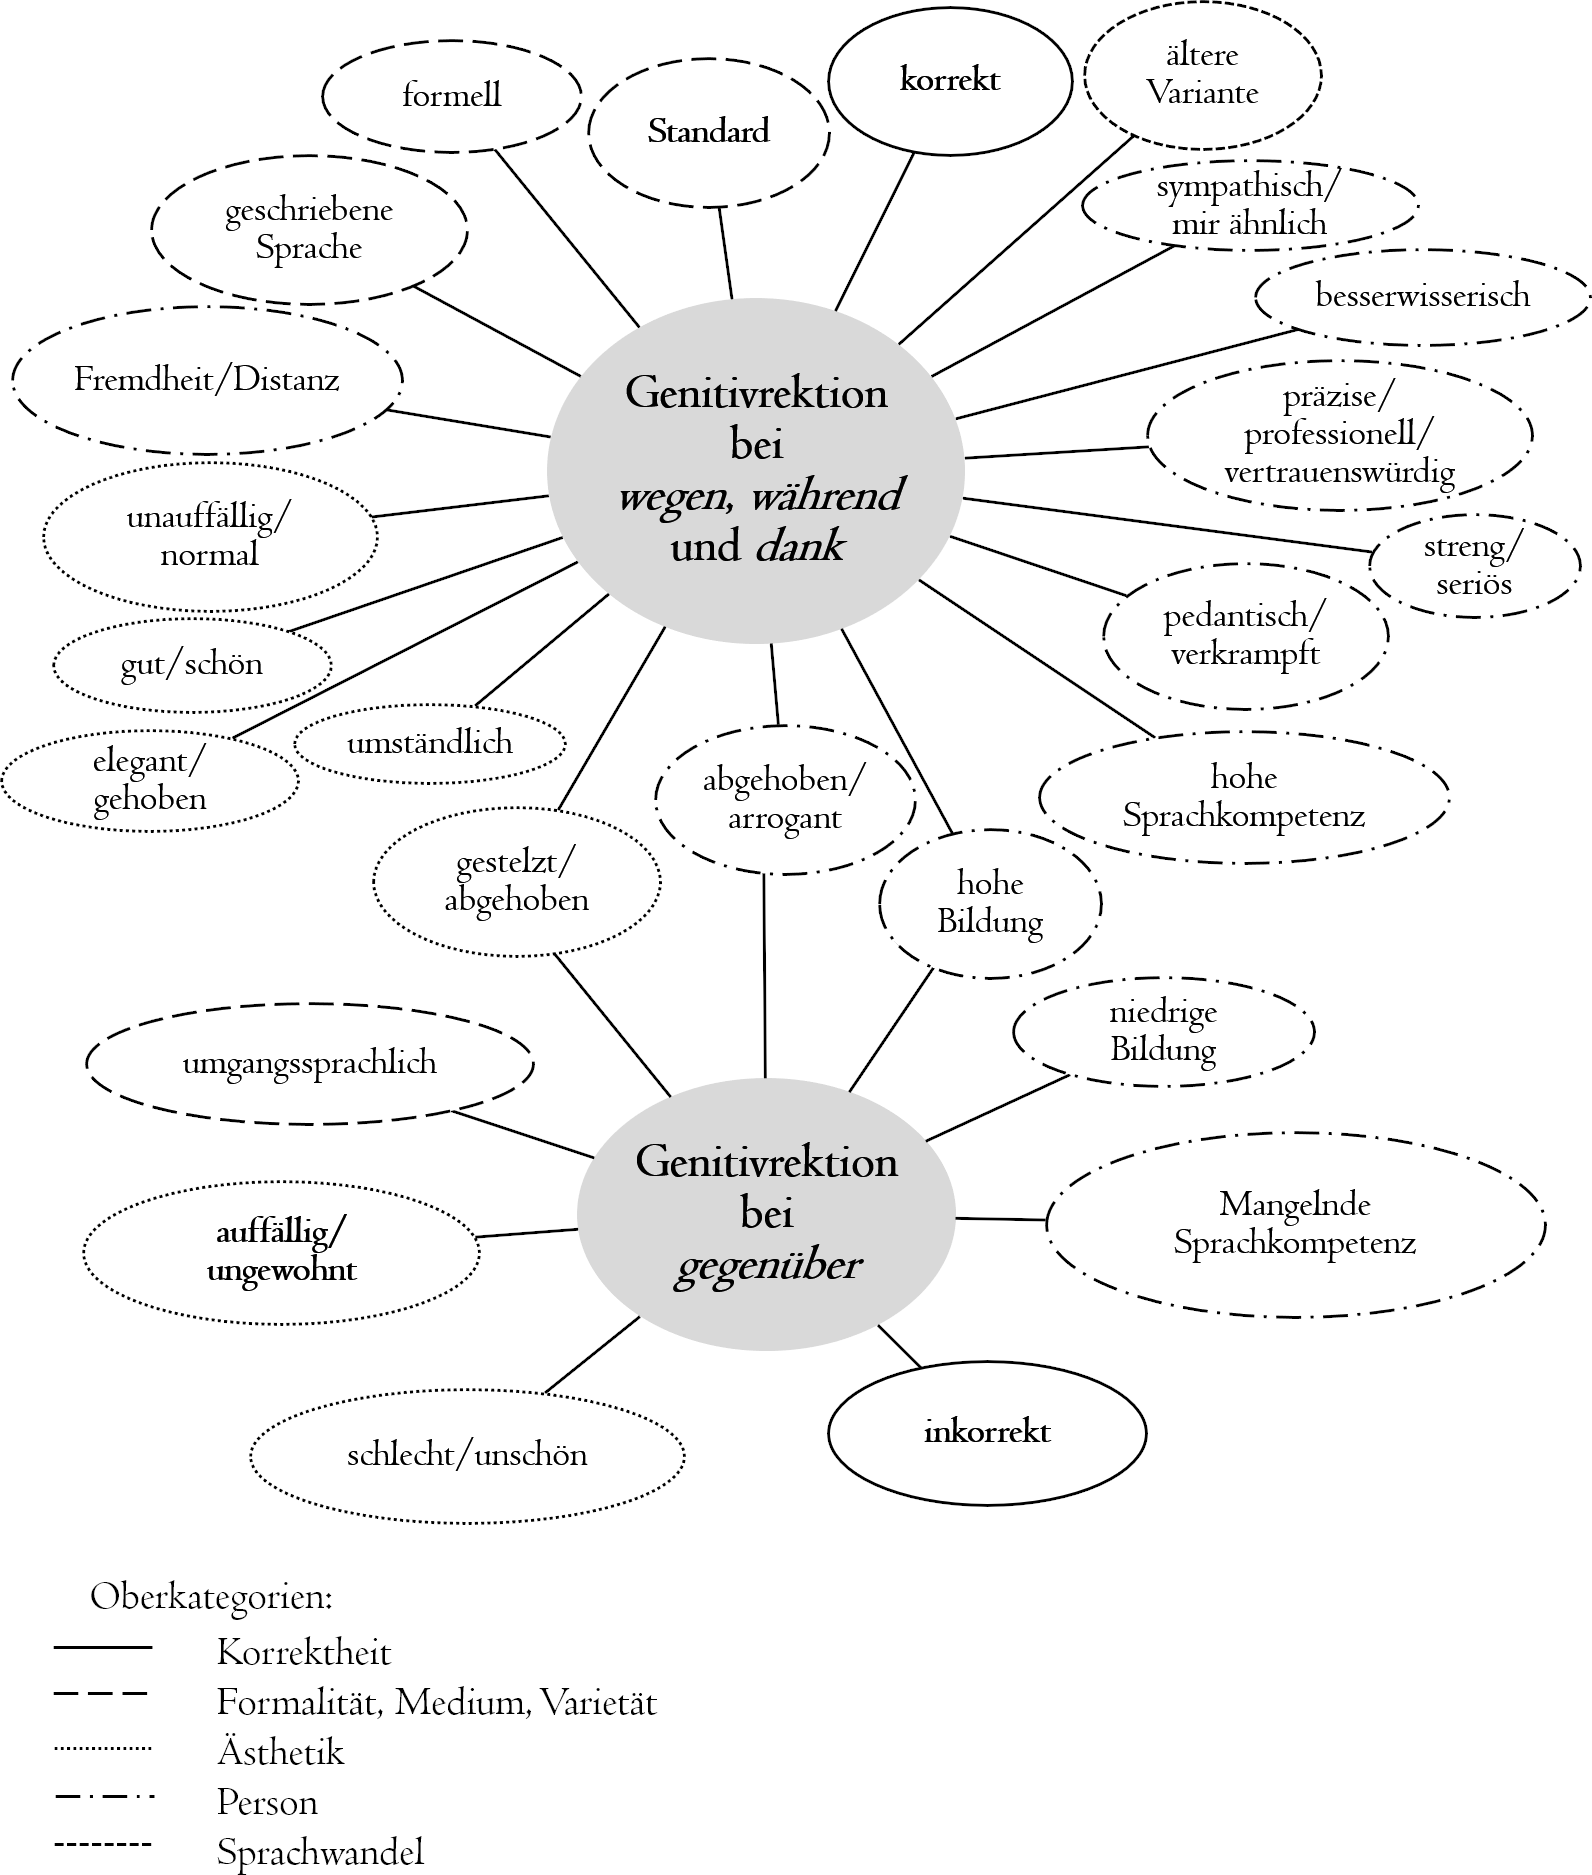
\includegraphics[width=\textwidth]{iFGenitiv.png}
\caption{Indexikalische Felder der Genitivrektion bei \wegen, \waehrend{} und \dank{} im Vergleich zu \gegenueber}
\label{pic:iFGenitiv}
\end{figure}

\newpage Im oberen Teil der Grafik sind die Zuschreibungen zu \wegen, \waehrend{} und \dank{} plus Genitiv zu sehen. 
Schon an der hohen Anzahl unterschiedlicher Kategorien lässt sich ablesen, dass die Indexikalität hier recht ausdifferenziert ist. 
Bei allen drei Präpositionen besteht die Variation zwischen Genitiv- und Dativrektion bereits über einen langen Zeitraum (\autoref{sec:Grammatikalisierung}), ebenso wie der Diskurs über diese Variation (\autoref{sec:IndexikalitaetRektionskasus}).
Die Kasusschwankung ist also schon lange Gegenstand metapragmatischer Reflexion, was zur Folge hat, dass sich die soziale Bedeutung der Varianten immer weiter auffächern konnte (\autoref{sec:Indexikalitaet}). 
Für die Bewertung macht es dabei kaum einen Unterschied, welche Rektionsvariante die sprachhistorisch ältere ist: 
Die Möglichkeit, dass eine Präposition ursprünglich den Dativ regierte, wird im Diskurs weitestgehend ausgeblendet (\autoref{sec:Prozesse}), wie man daran sieht, dass die Genitivrektion auch bei \dank{} als ältere und damit korrekte Variante konzeptualisiert wird (\autoref{sec:ErgAssSprachwandel}). 

\begin{sloppypar}
Die einzelnen indexikalischen Bedeutungen von \wegen, \waehrend{} und \dank{} mit dem Genitiv stehen untereinander in engem Zusammenhang.
Dies gilt insbesondere für die die Kategorien \glqq Standard\grqq{} und \glqq korrekt\grqq, die für die Konzeptualisierung der Varianten zentral sind:
%Auch Korrektheit und Standard selbst sind eng verwobene Assoziationskategorien:  
Aufgrund der verbreiteten Sprachideologie, die Standardsprache gelte als Zielnorm für alle Register, hat die Registrierung der Formen als standardsprachlich zur Folge, dass sie als korrekt bewertet werden (\autoref{sec:Prestigevarietaet}). 
Die eng verknüpften Kategorien \glqq korrekt\grqq{} und \glqq Standard\grqq{} ziehen die Assoziation mit anderen Kategorien nach sich und können daher als Kernkategorien verstanden werden.  
Mit der Standardsprachideologie hängt etwa die Beschreibung als \object{unauffällig} bzw. \object{normal} zusammen:
Die als Standard registrierten Varianten werden als Norm gesetzt. 
Da dem Standard außerdem positive ästhetische Werte zugeschrieben werden, lassen sich auch Verweise auf Werte wie \object{gut}, \object{schön}, \object{elegant} oder \object{gehoben} mit der Registrierung als standardsprachlich erklären (\autoref{sec:Prestigevarietaet}). 
Die Kategorien Korrektheit und angenehmer Klang bzw. angenehme Ästhetik, die sich bereits in anderen Studien als relevante Bewertungsgrößen bei Sprachurteilen herausgestellt haben (\autoref{sec:Bewertungsgrundlage}; s. \citealp{Preston2004}), lassen sich also auch in den Bewertungen der Rektionsvarianten von Sekundärpräpositionen wiederfinden.
Während in Untersuchungen zur Bewertung von Varietäten häufig festgestellt wurde, dass eine Varietät als ästhetisch und eine andere als korrekt empfunden wird \citep[s. etwa][53]{Preston2004}, werden bei den Rektionskasus allerdings sowohl Korrektheit als auch angenehmer Klang für die Genitivrektion beansprucht: 
Da die Standardsprache sowohl als korrekt als auch als ästhetisch gilt, ist die Genitivrektion über ihre Registrierung als standardsprachlich mit beiden Kategorien verknüpft. 
\end{sloppypar}


Mit der Beurteilung der Genitivrektion bei \wegen, \waehrend{} und \dank{} als standardsprachlich und korrekt hängt außerdem der Verweis auf Schriftlichkeit und Formalität eng zusammen. 
Dieser ist über kommunikative Praktiken zudem mit Fremdheit und Distanz zwischen den Kommunikationspartner:innen verknüpft: 
Formelle Schriftlichkeit ist metapragmatisch vor allem mit Situationen assoziiert, in denen die Kommunikationspartner:innen miteinander wenig vertraut sind.  
Damit ist wiederum der Verweis auf Personeneigenschaften verbunden, die in solchen Situationen relevant sind, etwa Professionalität, Vertrauenswürdigkeit und Seriosität. 
In anderen Situationen hingegen kann die Genitivrektion bei \wegen, \waehrend{} und \dank{} als pedantisch, verkrampft, abgehoben, arrogant oder besserwisserisch gewertet werden (\autoref{sec:ErgAssPersonen}). 
Insbesondere im Akzeptabilitätstest hat sich gezeigt, dass Befragte die Zusammenhänge zwischen der Wirkung einer Variante und dem Kontext, in dem sie auftaucht, sehr genau reflektieren: 
Zum einen wird die Angemessenheit von Dativ- und Genitivrektion bei \wegen{}, \waehrend{} und \dank{} in Abhängigkeit vom Setting bewertet (\autoref{sec:ErgAkzallg}), zum anderen begründen viele Befragte ihre Einschätzung einer Variante als unangemessen damit, dass sie im gegebenen Kontext einen negativen Eindruck zur Folge habe (\autoref{sec:Begruendungen}). 

Eine weitere relevante Kategorie, die mit den Genitivvarianten von \wegen, \waehrend{} und \dank{} in Verbindung gebracht wird, ist hohe Bildung.
Damit verknüpft ist auch die Vorstellung, dass Personen, die diese Varianten verwenden, sehr sicher im Umgang mit Sprache sind. 
Wie in \autoref{sec:Prestigevarietaet} ausgeführt, ist es typischerweise so, dass Varianten, die dem Standard zugeschrieben werden, auch als gebildet gelten. 
Gleichzeitig wird hohe Bildung mit Formalität und geschriebener Sprache in Verbindung gebracht, da Praktiken formeller Schriftlichkeit in Bildungsinstitutionen wie Schule und Universität gefordert und gelernt werden. 
In diesen Bedeutungszusammenhang lassen sich auch die oben bereits erwähnten Interpretationen als besserwisserisch oder pedantisch usw. einordnen. 
Als sympathisch wird die Genitivrektion bei \wegen{}, \waehrend{} oder \dank{} von Befragten empfunden, die sie in ihrem eigenen Sprachgebrauch verorten und daher eine Ähnlichkeit zu Personen feststellen, die diese Rektionsvariante ebenfalls verwenden (\autoref{sec:ErgAssPersonen}). 

Das indexikalische Bedeutungspotenzial der Variante \gegenueber{} plus Genitiv ist im unteren Teil von \autoref{pic:iFGenitiv} dargestellt. 
Es ist deutlich erkennbar, dass die Indexikalität hier weniger ausdifferenziert ist: 
Im Gegensatz zu den Präpositionen \wegen, \waehrend{} und \dank{} weist \gegenueber{} keine nennenswerte Variation in der Kasusrektion auf.
Dies kann ein Grund dafür sein, dass die Rektion dieser Präposition kaum metapragmatisch reflektiert wird (\autoref{cha:SekPraeps}). 
%\begin{figure}[h]
%\centering
%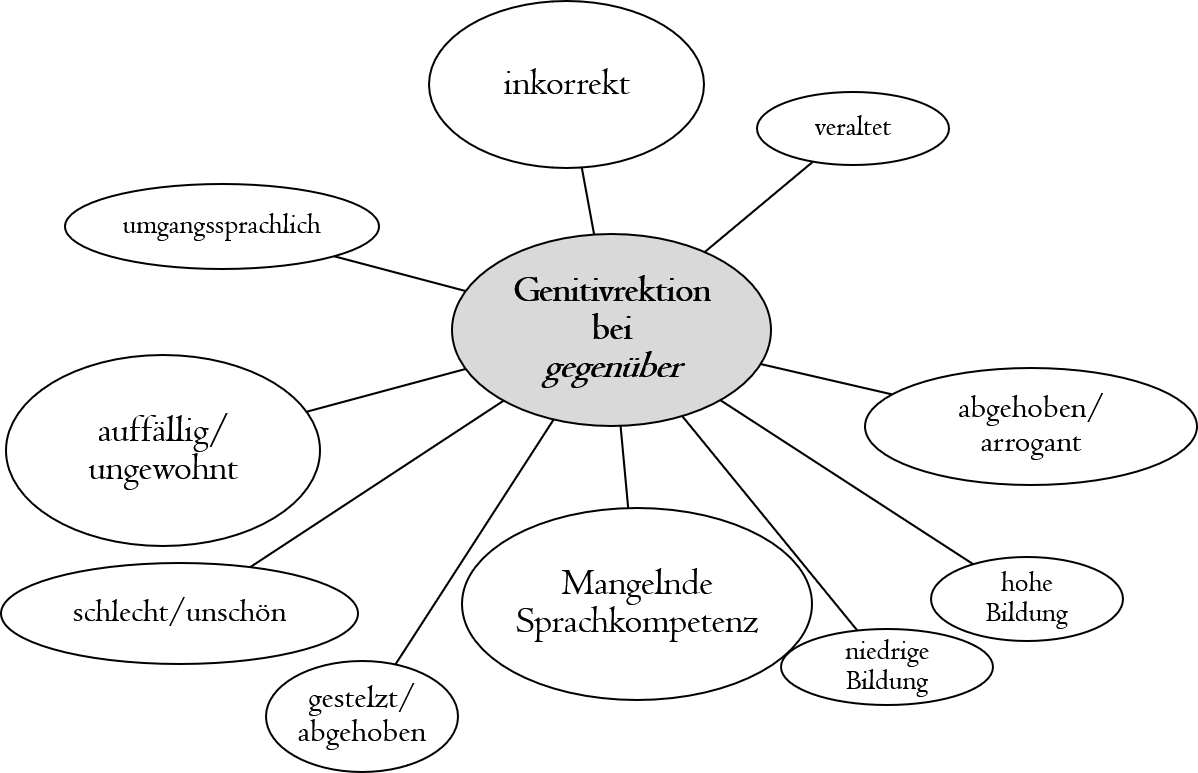
\includegraphics[scale=0.65]{iFGenitivGegenueber.png}
%\caption{Indexikalische Felder der Genitivrektion bei \gegenueber}
%\label{pic:iFGenitivGegenueber}
%\end{figure}

Die Auswertung der freien Assoziationen zu \gegenueber{} hat gezeigt, dass der Genitiv hier in erster Linie als inkorrekt, ungewohnt und auffällig bewertet wird (\autoref{sec:ErgAss}). 
Aus der Einstufung als sprachlich falsche Form folgt die Bewertung als schlecht und unschön (\autoref{sec:ErgAssAes}). 
Zudem wird die Verwendung von \gegenueber{} plus Genitiv als Anzeichen mangelnder Sprachkompetenz und niedriger Bildung gedeutet (\autoref{sec:ErgAssPersonen}). 
In einigen Äußerungen wird die Genitivrektion bei \gegenueber{} außerdem als missglückte Inszenierung von hoher Bildung gedeutet, wie in \autoref{sec:ErgAssPersonen} gezeigt. 
Anders als bei \wegen, \waehrend{} und \dank{} spielen die Kategorien Formalität und Medium bei \gegenueber{} keine Rolle. 
Statt als standardsprachlich wird die Genitivrektion hier als umgangssprachlich empfunden. 

Die klare Einordnung von \gegenueber{} plus Genitiv als von der Norm abweichendem Sprachgebrauch lässt sich auf das Frequenzwissen der Befragten zurückführen: 
Aufgrund ihrer Erfahrung wissen sie, dass diese Form nur sehr selten vorkommt. 
Die übrigen Eigenschaften, die der Variante zugeschrieben werden, lassen sich jedoch nicht auf diese Weise erklären: 
Bspw. wird die Genitivrektion bei \gegenueber{} ebenso wie bei \wegen, \waehrend{} und \dank{} als abgehoben, arrogant und gestelzt angesehen. 
Diese Assoziationen lassen sich nur aus dem Diskurswissen der Befragten herleiten: 
Im Diskurs um Präpositionen mit Kasusschwankungen wie etwa \wegen{} werden dem Genitiv bestimmte Eigenschaften zugeschrieben, bspw. hohe Bildung.
Diese Zuschreibungen werden von einigen Befragten auf die Genitivrektion bei \gegenueber{} übertragen. 
Dazu trägt wahrscheinlich bei, dass die Genitiv- und die Dativrektion bei \gegenueber{} im Fragebogen als gleichwertige Varianten nebeneinander präsentiert werden, sodass bei den Befragten der Eindruck entstehen kann, hier liege ein ähnlicher Variationsfall vor wie bei prominenten Diskursbeispielen wie \wegen. 

Die teilweise widersprüchlichen Assoziationen zu \gegenueber{} mit dem Genitiv deuten darauf hin, dass Befragte durch die Konfrontation mit dieser an sich ungebräuchlichen Variante verunsichert werden. 
Dies bestätigt die Auswertung der Frage danach, wie sicher sich die Befragten bei ihrer Antwort sind. 
Dieser Teil des Akzeptabilitätstest wurde in der vorliegenden Untersuchung ausgespart und in \citet[][]{Vieregge.2019b} veröffentlicht: 
Während bei den schwankenden Präpositionen \wegen, \waehrend{} und \dank{} jeweils über 80\,\% der Befragten angeben, sie seien in der Bewertung der Akzeptabilität sicher, sind es bei den Präpositionen \gegenueber{} und \object{seit} etwas weniger \citep[s.][88--90]{Vieregge.2019b}.\footnote{Gefragt wurde jeweils \glqq wie sicher sind Sie sich bei Ihrer Antwort?\grqq{} und die Befragten konnten zwischen folgenden Antwortmöglichkeiten wählen: ganz sicher, ziemlich sicher, etwas unsicher, sehr unsicher.} 
Die Unsicherheit könnte auch erklären, warum die Anzahl der Befragten, die \gegenueber{} und \object{seit} mit dem Genitiv als korrekt und angemessen beurteilen, jeweils größer ist als die Anzahl derer, die angeben, diese Formen selbst zu verwenden (\autoref{sec:ErgAkzallg}). 

In \autoref{pic:iFDativ} sind die indexikalischen Felder von \wegen, \waehrend{} und \dank{} plus Dativ sowie von \gegenueber{} plus Dativ visualisiert. 
Die Dativrektion bei \wegen, \waehrend{} und \dank{} wird ebenso wie die Genitivrektion bei diesen Präpositionen stark reflektiert und verfügt daher über ein ausdifferenziertes Set an indexikalischen Bedeutungen, das im oberen Teil der Grafik dargestellt ist. 
Es fällt auf, dass die Bedeutungen, die dem Dativ zugeschrieben werden, Gegensatzpaare mit den Zuschreibungen zur Genitivrektion bilden:
Während der Genitiv als korrekt, formell und schriftsprachlich gilt, wird die Dativrektion bei \wegen, \waehrend{} und \dank{} als inkorrekt, informell und gesprochensprachlich bezeichnet.
Sie wird zudem nicht mit der Standardsprache in Verbindung gebracht, sondern mit Umgangs- und Alltagssprache sowie Regionalsprache und Dialekt (\autoref{sec:ErgAssFormMedVar}). 

In der Bewertung der Dativrektion stellt die Einordnung als inkorrekt eine Kernkategorie dar, die mit anderen Zuschreibungen eng verknüpft ist: 
Die Vorstellung, umgangssprachlicher oder dialektaler Sprachgebrauch sei fehlerhaft, ist eine verbreitete Sprachideologie (\autoref{sec:Einheitlichkeit}). 
Auch negative ästhetische Eigenschaften wie schlecht, unschön oder plump werden Formen, die vom Standard abweichen und daher die vermeintliche Einheitlichkeit der Sprache bedrohen, häufig zugesprochen. 
Das gilt insbesondere für Formen, die wie \wegen, \waehrend{} und \dank{} plus Dativ als Resultat eines unerwünschten Sprachwandels wahrgenommen werden (\autoref{sec:ErgAssSprachwandel}). 

\begin{figure}[hp]
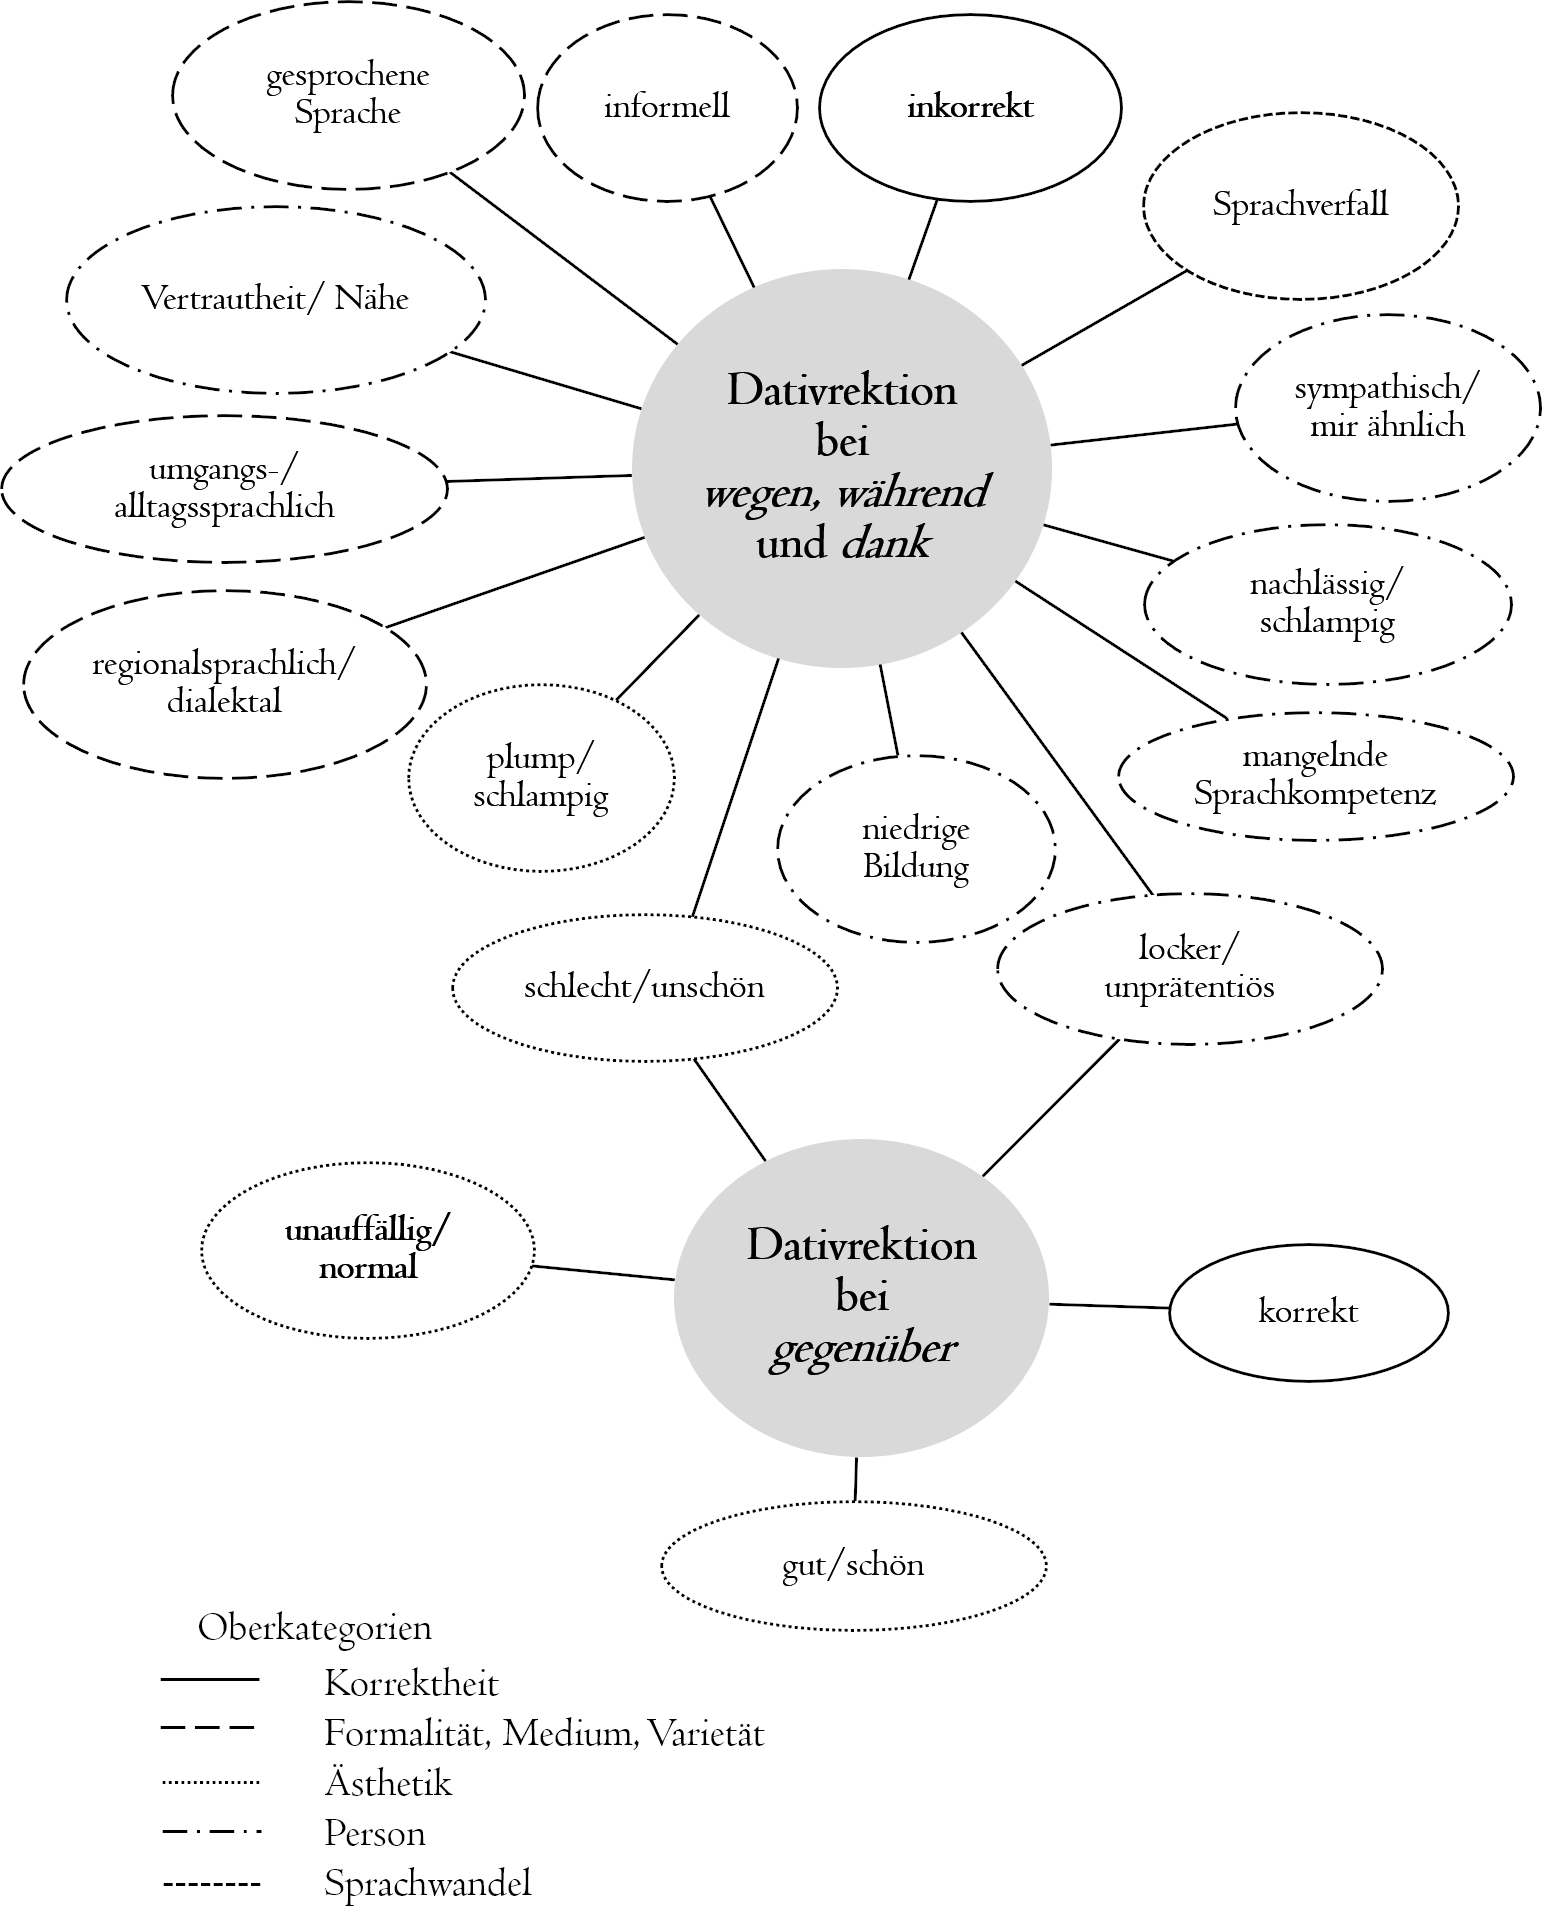
\includegraphics[width=\textwidth]{iFDativ.png}
\caption{Indexikalische Felder der Dativrektion bei \wegen, \waehrend{} und \dank{} im Vergleich zu \gegenueber}
\label{pic:iFDativ}
\end{figure}

Die konträren Zuschreibungen zur Genitiv- und Dativrektion bei \wegen, \waehrend{} und \dank{} machen deutlich, wie die Rektionsvariation zur Differenzierung zwischen sozialen Gruppen und Personentypen genutzt wird. 
So steht der Dativ im Gegensatz zum Genitiv für niedrige Bildung und mangelnde Sprachkompetenz (\autoref{sec:ErgAssPersonen}). 
Neben einem geringen Bildungsniveau wird als Ursache für seinen Gebrauch Nachlässigkeit vermutet. 
Außerdem gilt er als locker und unprätentiös und wird mit Situationen assoziiert, in denen die Kommunikationspartner:innen sich nahe stehen. 

Sowohl die Genitivrektion als auch die Dativrektion bei \wegen, \waehrend{} und \dank{} werden als sympathisch empfunden. 
Dies liegt vermutlich daran, dass Befragten häufig die Variante als sympathisch gilt, von der sie sagen, dass sie sie selbst verwenden (\autoref{sec:ErgAssPersonen}). 
Der Sprachgebrauch einer Person ist ihnen also aufgrund der (vermeintlichen) Ähnlichkeit zu ihrem eigenen Sprachgebrauch vertraut und daher sympathisch.  

Mit der Dativrektion bei \gegenueber{} assoziieren die Befragten kaum spezifische Kontexte oder Personentypen, wie im unteren Teil von \autoref{pic:iFDativ} erkennbar.
Die zentrale Assoziationskategorie ist hier \glqq unauffällig/normal\grqq. 
Die Form wird daneben vor allem als korrekt bezeichnet, teilweise auch als gut oder schön (\autoref{sec:ErgAssKorrektheit} und \autoref{sec:ErgAssAes}). 
Dies lässt sich darauf zurückführen, dass bei \gegenueber{} kaum Variation vorliegt und die Dativrektion wenig salient erscheint. 
Anders als bei \gegenueber{} plus Genitiv werden Befragte hier daher offenbar kaum dazu veranlasst, auf ihr Diskurswissen über die Rektionsvariation bei Sekundärpräpositionen zurückzugreifen.  
Andeutungsweise findet sich dieses lediglich in den Eigenschaftszuschreibungen locker und unprätentiös sowie in den ästhetischen Urteilen schlecht und unschön. 
Letztere stehen im Gegensatz zu den oben erwähnten positiven ästhetischen Zuschreibungen und könnten damit evtl. auf eine Diskrepanz zwischen dem Diskurswissen um den Dativ und der Unauffälligkeit dieses Kasus bei \gegenueber{} hindeuten. 
%\begin{figure}[h]
%\centering
%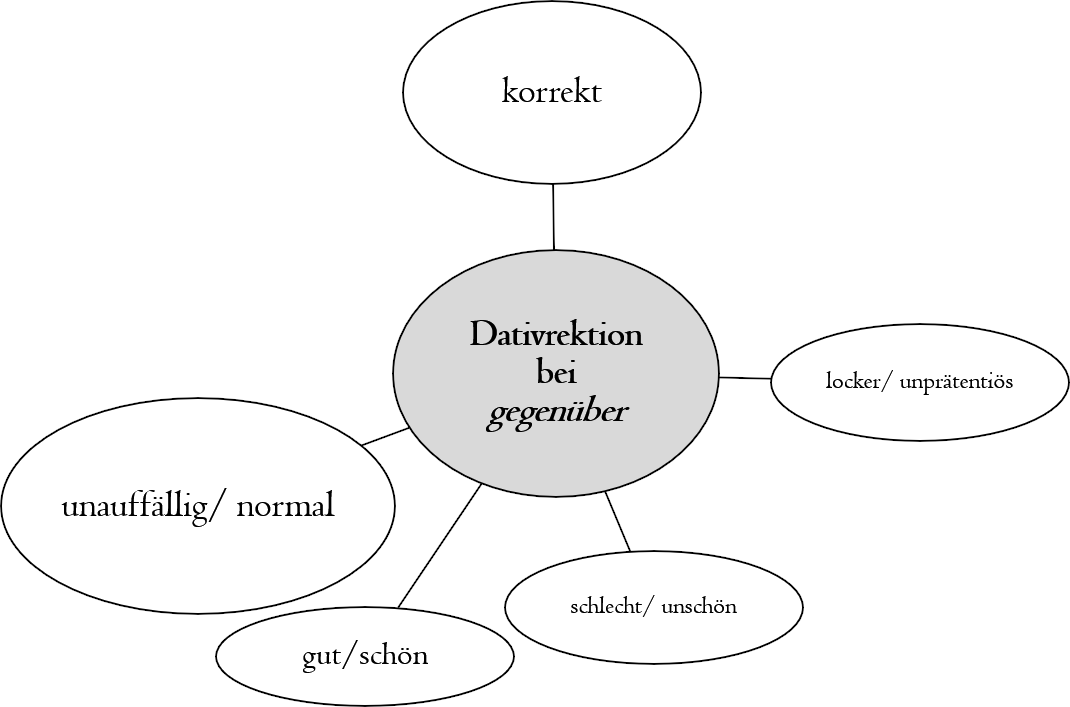
\includegraphics[scale=0.65]{iFDativGegenueber.png}
%\caption{Indexikalische Felder der Dativrektion bei \gegenueber}
%\label{pic:iFDativGegenueber}
%\end{figure}

Die Modellierung der indexikalischen Felder macht deutlich, dass es zu kurz greift, die Genitivrektion pauschal als Prestigevariante zu deuten und die Dativrektion als stigmatisiert: 
Beide Varianten verfügen über ausdifferenzierte Sets indexikalischer Bedeutungen. 
Dabei sind die Bedeutungszuschreibungen nicht willkürlich, sondern ideologisch durchformt.
Dies ist an der Relevanz von Kategorien wie Korrektheit oder Standardsprachlichkeit erkennbar, die auch zahlreiche andere metapragmatische Diskurse prägen (\autoref{sec:Bewertungsgrundlage}). 
Auch die Argumentation mit ästhetischen Eigenschaften sowie die Unterscheidung in eine gebildete und eine ungebildete Variante tauchen in sprachideologischen Diskursen immer wieder auf. 

Ein wichtiges Ergebnis der Studie ist, dass für Indexikalität nicht allein der Rektionskasus entscheidend ist, sondern auch, mit welcher Sekundärpräposition dieser gebraucht wird. 
Dies zeigt sich daran, dass die Varianten der Präposition \gegenueber{}, die in ihrer Rektion kaum schwankt, anders bewertet werden als die Varianten von \wegen, \waehrend{} und \dank. 

Welche sozialen Bedeutungen einer Variante aktiviert werden, ist von verschiedenen Kontextmerkmalen abhängig. 
Hier zeigt sich der sprachideologische Prozess der fraktalen Rekursivität (\autoref{sec:Prozesse}): 
Die beiden von \citet{Silverstein2003} beschriebenen Aspekte der Indexikalität (\autoref{sec:Indexikalitaet}), also die Angemessenheit  in einem bestimmten Kontext (\textit{presupposition}) und die Wirkung in diesem Kontext (\textit{entailment}), basieren bei den Rektionsvarianten in hohem Maße auf durch fraktale Rekursivität entstandenen Zuschreibungen. 
Zunächst werden Oppositionen wie Standard vs. Nonstandard und korrekt vs. inkorrekt auf die Opposition zwischen den beiden Rektionsvarianten projiziert. 
Innerhalb einer Variante wird jedoch weiter differenziert. 
So hat sich im Akzeptabilitätstest gezeigt, dass die Dativrektion bei \wegen{} und \waehrend{} in informellen Kontexten von vielen Befragten als inkorrekt, aber dennoch angemessen gewertet wird (\autoref{sec:ErgAkzallg}). 
Hier wird der Standard zwar als Zielnorm herangezogen, es besteht jedoch auch das Bewusstsein, dass je nach Register unterschiedliche Varianten verwendet werden können. 
Dieses Ergebnis könnte zu einem gewissen Grad vom Studiendesign beeinflusst sein:
Die getrennte Abfrage von Korrektheit und Angemessenheit könnte die Diskrepanz in der Bewertung erst hervorgebracht haben, da durch die Gegenüberstellung impliziert wird, dass es hier Unterschiede gibt \citep[s.][190]{Wolfer.2020}. 
Jedoch zeigen die freien Antworten im Assoziationsteil, der dem Akzeptabilitätstest vorausgeht, dass die Befragten von sich aus zwischen korrekt und angemessen differenzieren (\autoref{sec:ErgAss}). 
Bspw. wird der Genitiv in informellen Situationen teilweise als arrogant und daher unpassend gewertet. 

Der folgende Abschnitt widmet sich der Frage, welches Erklärungspotenzial die Indexikalität der untersuchten Rektionsvarianten für ihre Verwendung hat. 
\section[Erklärungspotenzial der Indexikalität]{Erklärungspotenzial der Indexikalität für die Verwendung der Rektionsvarianten}
\label{sec:DiskVariationundWandel}
Im Theorieteil der Studie wurde ausgeführt, dass die Kasuswahl bei Sekundärpräpositionen sich nicht allein mit der fortschreitenden Grammatikalisierung dieser Präpositionen erklären lässt (\autoref{sec:Grammatikalisierung}). 
Daher richtet die vorliegende Untersuchung den Blick auf den Einfluss der metapragmatischen Bewertung von Genitiv und Dativ auf die Verwendung der Rektionskasus. 

Die im Fragebogen erhobenen Produktionsdaten bestätigen das mangelnde Erklärungspotenzial der Grammatikalisierungstheorie: 
Die beiden ursprünglichen Genitivpräpositionen \wegen{} und \waehrend{} werden überwiegend mit dem Genitiv gebraucht (\autoref{sec:ErgProduktion}). 
Obwohl die Variation zwischen Genitiv und Dativ hier bereits lange besteht, setzt sich der für Präpositionen des Deutschen typische Dativ nicht durch. 
Das heißt auch, dass die Kasusrektion nicht zur Differenzierung von der Spenderstruktur genutzt wird (\autoref{sec:Differenzierung}). 
Die ursprüngliche Dativpräposition \dank{} ist hingegen zur Genitivrektion übergegangen: 
Im Produktionsexperiment entscheidet sich die große Mehrheit der Befragten für \dank{} plus Genitiv. 
Hier hat sich die Differenzierung über die Kasusrektion also sehr schnell vollzogen. 
Da \dank{} dabei von der Dativ- zur Genitivrektion wechselt, bedeutet dies eine Entfernung vom Prototyp. 
Dass diese schneller vonstatten geht als die Annäherung an den Prototyp bei \wegen{} und \waehrend{}, die gleichzeitig eine Differenzierung von den Sprenderstrukturen bedeuten würde, lässt sich grammatikalisierungstheoretisch nicht erklären. 

Die sprachhistorisch junge Präposition \gegenueber{} kommt in Korpora bisher beinahe ausschließlich mit dem Dativ vor (\autoref{sec:Differenzierung}). 
Dennoch gebraucht ungefähr ein Zehntel der Befragten die Genitivrektion im Produktionsexperiment.
Dass dieser Anteil nicht zu vernachlässigen ist, zeigt der Vergleich mit den anderen Präpositionen: 
Der Anteil der Befragten, der \gegenueber{} mit dem Genitiv verwendet, entspricht dem Anteil der Befragten, der \waehrend{} und \dank{} im formellen Lückentext mit dem Dativ gebraucht. 
Die leichten Kasusschwankungen bei \gegenueber{} können evtl. als erste Anzeichen einer fortschreitenden Differenzierung der Präposition von ihrer Spenderstruktur gesehen werden. 
Mit dieser Interpretationsweise lässt sich jedoch nicht erklären, warum der Genitivanteil bei \gegenueber{} in Befragungen höher ist als in Korpora (vgl. auch die Ergebnisse von \citealp{Becker2011}). 
Noch überraschender als der Genitivanteil bei \gegenueber{} ist, dass im formellen Teil des Produktionsexperiments eine ähnlich hohe Anzahl Befragter die Genitivrektion bei der Primärpräposition \object{seit} verwendet.
Da Primärpräpositionen am Ende der Grammatikalisierungsskala stehen, sollte es hier nicht zu Kasusschwankungen kommen (\autoref{sec:Sekundaer}). 
Dass der Genitiv sogar bei \object{seit} auftaucht, deutet bereits darauf hin, dass bei der Kasuswahl weitere Faktoren eine wesentliche Rolle spielen müssen. 

Für die beschriebenen Tendenzen bei der Verwendung der Rektionsvarianten im Produktionsexperiment reicht das Erklärungspotenzial der Grammatikalisierungstheorie nicht aus. 
Aus diesem Grund wird in dieser Studie die Indexikalität von Genitiv und Dativ als zentraler Steuerungsfaktor für die Verwendung der Rektionsvarianten vorgeschlagen. 
So kann bspw. die starke Tendenz zum Genitiv, die bei \wegen{}, \waehrend{} und \dank{} zu beobachten ist, damit erklärt werden, dass dieser Kasus als standardsprachlich und korrekt gilt. 
Da die hier vorgestellte Umfrage erkennbar von einer Universität stammt und von einigen sogar als Testsituation empfunden wird (\autoref{sec:ErgProdInfForm}), verwenden Befragte Genitivvarianten hier eher als die Dativvarianten, die als inkorrekt und nicht standardsprachlich registriert sind. 
Damit positionieren sie sich gegenüber der Forscherin und der Institution, der sie angehört (\autoref{sec:Positionierung}; vgl. das Positionierungsmodell von \citealp{Spitzmuller2013}). 
Die Genitivrektion verweist indexikalisch auf einen Personentypus, der sich unter anderem durch hohe Bildung, Kompetenz und Professionalität auszeichnet, sowie auf Situationen, in denen Standardsprache und formelle Schriftlichkeit verwendet werden. 
Wie oben bereits erwähnt, sind diese indexikalischen Bedeutungen untereinander eng verknüpft. 
Indem Befragte die Genitivrektion verwenden, zeigen sie ihre affirmierende Einstellung zu den mit diesem Kasus verbundenen Werten und signalisieren ihre Zugehörigkeit zum Personentypus \glqq gebildete Person\grqq{}. 
Sie inszenieren sich also als gebildet, professionell und kompetent. 
Damit richten sie sich gleichzeitig gegenüber der Forscherin aus: 
Diese entspricht aus Sicht der Befragten als Angehörige einer Universität dem mit dem Genitiv assoziierten Personentypus. 
Zudem werden Forschung und Universitäten meist mit Standardsprache, Formalität und Schriftlichkeit verknüpft, weshalb die Befragten vermutlich davon ausgehen, dass die Forscherin sich diesen Registern gegenüber positiv positioniert. 
%\begin{figure}[h]
%\centering
%\includegraphics[scale=0.55]{PositionierungProd.png}
%\caption{Positionierung der Befragten durch Verwenden der Genitivrektion im Produktionsexperiment \citep[nach][]{Spitzmuller2013}}
%\label{pic:PositionierungProd}
%\end{figure}

\begin{sloppypar}
Die Analyse der Kasuswahl im Produktionsexperiment als Positionierung macht deutlich, wie relevant es ist, Fragebogendaten als Teil einer Interaktion zu interpretieren (\autoref{sec:Methodologie}).
Das gilt in gleichem Maße für die Antworten im Assoziationsteil sowie im Akzeptabilitätsteil des Fragebogens:
Noch expliziter als durch die eigene Verwendung einer Variante können sich Befragte positionieren, indem sie eine Variante in eigenen Worten oder durch Auswahl einer Option wie \glqq angemessen\grqq{} bzw. \glqq nicht angemessen\grqq{} bewerten. 
\end{sloppypar}

Wie bereits bei der metapragmatischen Bewertung der untersuchten Rektionsvarianten wird die Relevanz der Kategorie \glqq Formalität\grqq{} auch in der Verwendung der Varianten im Produktionsexperiment deutlich: 
Die Präpositionen \wegen{}, \waehrend{} und \dank{} werden im informellen Lückentext deutlich häufiger mit dem Dativ gebraucht als im formellen Lückentext (\autoref{sec:ErgProdInfForm}).
Dies bestätigt Ergebnisse aus Korpusuntersuchungen, in denen sich ebenfalls ein registerspezifischer Gebrauch der Kasus abzeichnet (\autoref{sec:KorpusstudienRektion}).
Die für die vorliegende Studie erhobenen expliziten metapragmatischen Äußerungen zu den Rektionsvarianten belegen, dass diese Verteilung von Sprachbenutzer:innen reflektiert wird: 
Sie deuten die Varianten als Kontextualisierungshinweise für formelle oder informelle Situationen (\autoref{sec:ErgAssFormMedVar}; \autoref{sec:Begruendungen}).  
%Es handelt sich also nicht um Indexikalität der ersten Ordnung (\autoref{sec:Indexikalitaet}), bei der die Verteilung der Varianten auf unterschiedliche Register den Sprachbenutzer:innen nicht bewusst ist, sondern um Indexikalität der zweiten oder dritten Ordnung: 
Der unterschiedliche Kasusgebrauch im formellen und im informellen Lückentext stützt die Hypothese, dass die Befragten die Rektionsvarianten darüber hinaus selbst als Kontextualisierungshinwese einsetzen. 
Anders ist dies bei der wenig grammatikalisierten Präposition \gegenueber{}:
Hier sind die Rektionsvarianten kaum indexikalisiert und werden auch nicht als Kontextualisierungshinweise genutzt. 
Bei der Primärpräposition \object{seit} lassen sich ebenfalls keine Unterschiede zwischen dem formellen und dem informellen Lückentext feststellen. 
 
Auch regionale Unterschiede, die bereits in Korpusuntersuchungen sichtbar geworden sind (s. \cites{Petig1997}{Elter2005}; \autoref{sec:KorpusstudienRektion}), finden sich in den Produktionsdaten (\autoref{sec:ErgProdNachHerkunft}; \autoref{sec:ErgProdCTrees}): 
Bei \wegen{}, \waehrend{} und \dank{} wird der Dativ von süddeutschen Befragten häufiger verwendet als von norddeutschen (\autoref{sec:ErgProdNachHerkunft}; \autoref{sec:ErgProdCTrees}). 
Hierin spiegelt sich die unterschiedliche Bewertung der Rektionskasus in den verschiedenen Regionen Deutschlands:
Insbesondere im informellen Setting des Akzeptabilitätstests wird die Dativrektion bei \wegen{} und \waehrend{} von Befragten aus Süddeutschland häufiger als angemessen beurteilt als von Befragten aus Norddeutschland (\autoref{sec:ErgAkzNachRegion}; \autoref{sec:ErgAkzCTrees}). 
Bei \gegenueber{} und \object{seit} zeigen sich solche regionalen Unterschiede nicht. 

Dass die Beschreibung der Kasusschwankungen bei den hier untersuchten Präpositionen als Begleiterscheinung ihrer Grammatikalisierung zu kurz greift, wird nicht zuletzt auch daran deutlich, dass ältere Befragte nicht unbedingt die ältere {Rektions\-va\-rian\-te} einer Präposition verwenden, wie es bei einem Sprachwandelphänomen evtl. erwartet werden könnte \citep[s.][40]{Preston.1991}. 
Stattdessen ist auch hier die Indexikalität entscheidend, sodass die Variante \dank{} plus Genitiv, von der angenommen wird, sie sei älter, unter älteren Befragten akzeptabler bewertet und häufiger verwendet wird als \dank{} plus Dativ (\autoref{sec:ErgAkzNachAlter}; \autoref{sec:ErgProdNachAlter}). 

Insgesamt verdeutlichen die Ergebnisse, dass metapragmatische Bewertung % Änderung Anfang 
und Variation % Änderung Ende und Wandel 
der Rektion von Sekundärpräpositionen nicht getrennt voneinander gedacht werden können: 
Die voranschreitende Grammatikalisierung der Präpositionen löst Kasusschwankungen aus, die von Sprachbenutzer:innen reflektiert und mit sozialer Bedeutung aufgeladen werden. 
Diese Indexikalisierung der Rektionskasus beeinflusst ihre Verwendung in konkreten Interaktionssituationen. 

Im folgenden Kapitel wird ein Ausblick gegeben, wie an die Ergebnisse der vorliegenden Studie mit weiteren Untersuchungen angeknüpft werden kann. 
%Erklärung für häufigeren Genitivgebrauch unter Hochschulabsolvent:innen: 
%Die Vermutung, dass Befragte ohne Hochschulabschluss den Genitiv häufiger mit negativen Werten assoziieren und ihn deswegen seltener verwenden, lässt sich anhand der Daten nicht bestätigen: 
%Assoziationen mit Eigenschaften wie Arroganz oder Verkrampftheit werden in beiden Bildungsgruppen geäußert.
%Bei gegenueber und seit wählen außerdem mehr Leute ohne HSA den Genitiv!
%Da, wo der Genitiv innovativ ist, wird er eher von Jüngeren und Leuten ohe HSA verwendet... %Muss noch ausführlicher erklärt werden! Z.B. Zusammenhang mit Normbewusstsein (s. Kommentar JF)
